\subsection{Problem}

\renewcommand{\theequation}{\theenumi}
\begin{enumerate}[label=\thesection.\arabic*.,ref=\thesection.\theenumi]
\numberwithin{equation}{enumi}
\item Sketch circles with equation:
The following python codes generate the required circles :
	\begin{lstlisting}
	./codes/circle/q18abc.py
	./codes/circle/q18d.py
	\end{lstlisting}


\begin{enumerate}

\item \begin{multline} 
\vec{x^Tx} - \myvec{4\\8}\vec{x} -45 = 0\text{ represented in Fig:\ref{fig:qoeabc}}
\\
\text{Center is }\myvec{2\\4}\quad\text{Radius is }\sqrt{65}
\end{multline}

	\begin{figure}[!ht]
	\centering
	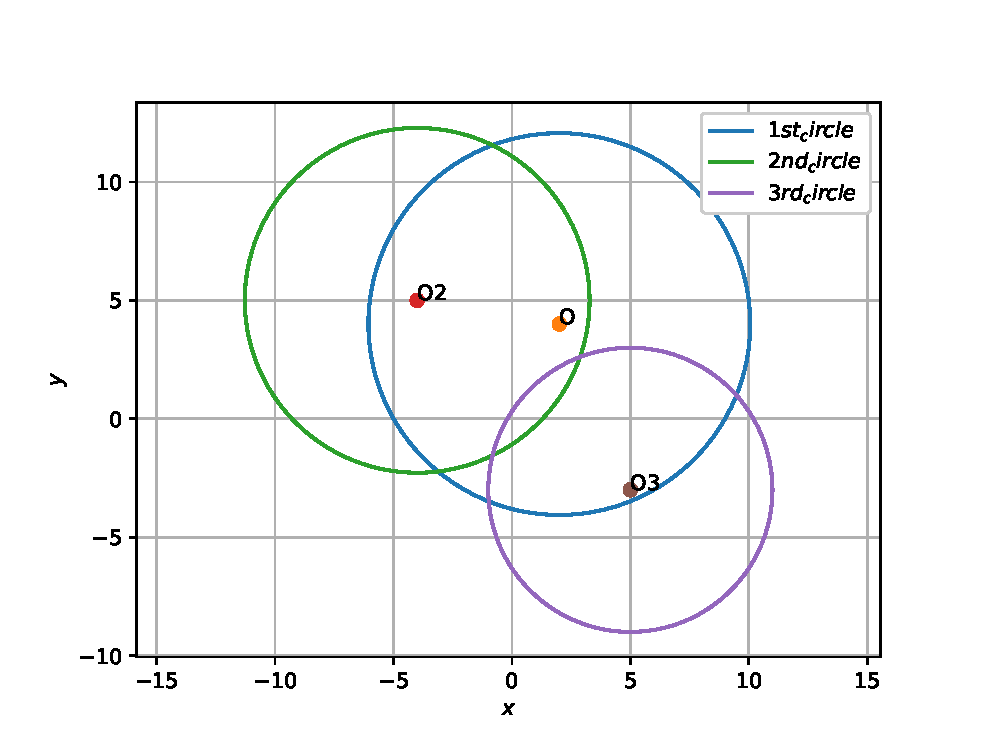
\includegraphics[width=\columnwidth]{./figs/circle/q18abc.eps}
	\caption{Circle of Q.4.2.5}
	\label{fig:qoeabc}	
	\end{figure}

\item \begin{multline} 
\vec{x^Tx} - \myvec{8\\-10}\vec{x} - 12 = 0\text{ represented in Fig:\ref{fig:qoeabc}}
\\
\text{Center is }\myvec{-4\\5}\quad\text{Radius is }\sqrt{53}
\end{multline}


\item \begin{multline} 
\norm{x - \myvec{5\\-3}} = 36\text{ represented in Fig:\ref{fig:qoeabc}}
\\
\text{Center is }\myvec{5\\-3}\quad\text{Radius is }6
\end{multline}



\begin{comment}
	\begin{figure}[!ht]
	\centering
	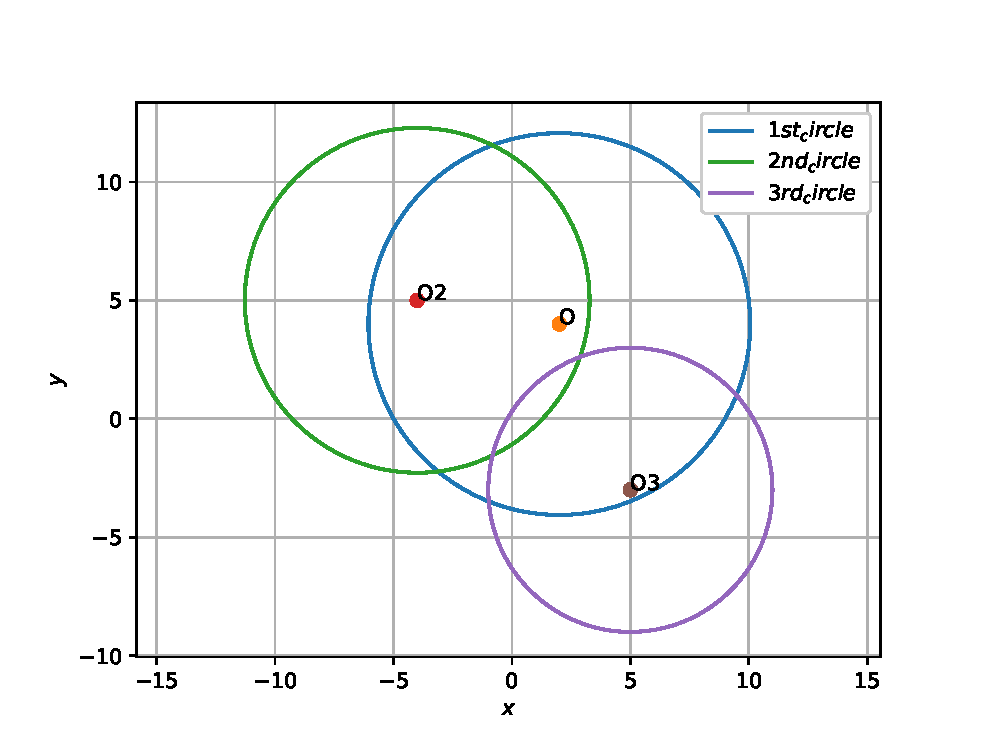
\includegraphics[width=\columnwidth]{./figs/circle/q18abc.eps}
	\caption{Circle of Q.4.2.5}
	\label{fig:qoeb}	
	\end{figure}
\end{comment}
\begin{comment}
	\begin{figure}[!ht]
	\centering
	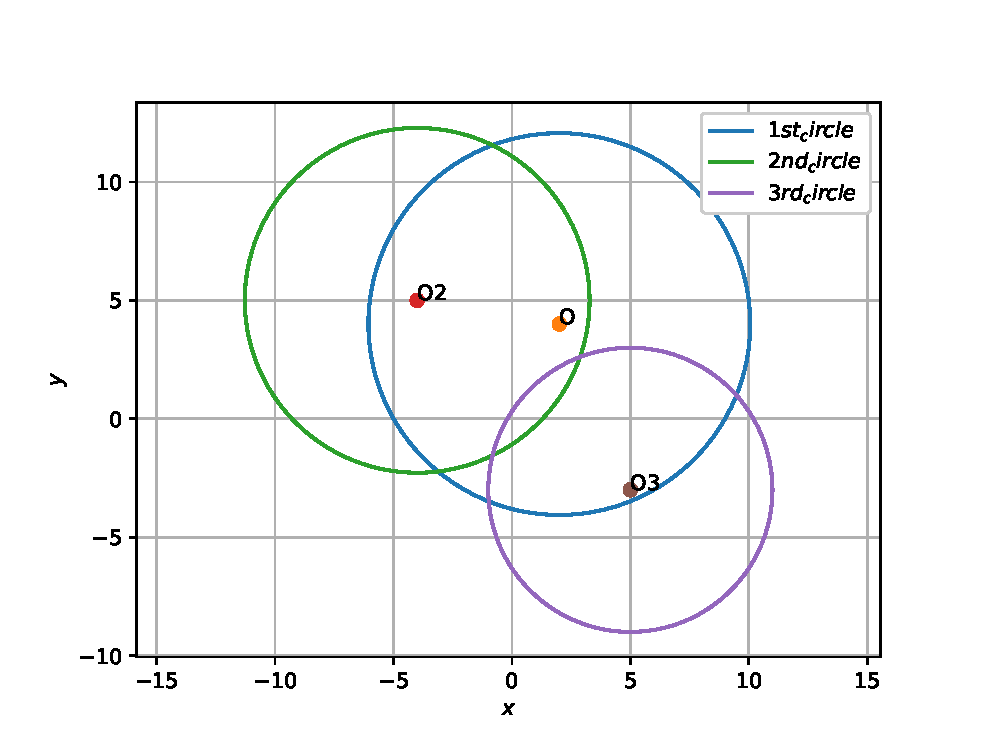
\includegraphics[width=\columnwidth]{./figs/circle/q18abc.eps}
	\caption{Circle of Q.4.2.5}
	\label{fig:qoec}	
	\end{figure}
\end{comment}
\item \begin{multline} 
2\vec{x^Tx} - \myvec{1\\0}\vec{x} = 0\text{ represented in Fig:\ref{fig:qoed}}
\\
\text{Center is }\myvec{0.25\\0}\quad\text{Radius is }0.25
\end{multline}
	\begin{figure}[!ht]
	\centering
	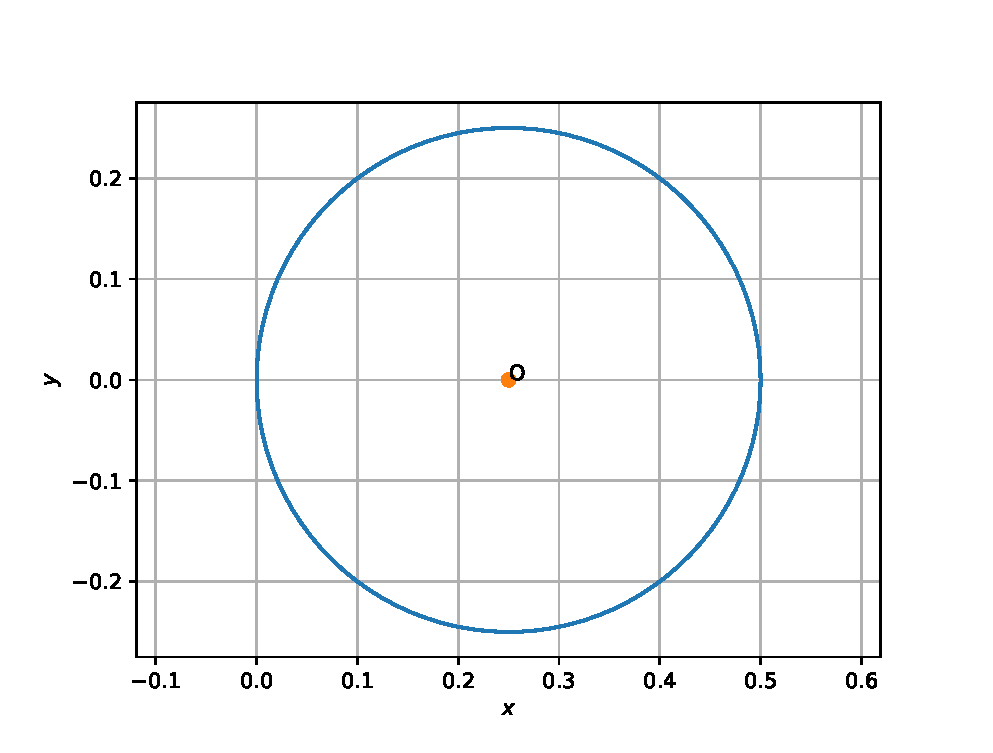
\includegraphics[width=\columnwidth]{./figs/circle/q18d.eps}
	\caption{Circle of Q.4.2.5}
	\label{fig:qoed}	
	\end{figure}



\end{enumerate}
\end{enumerate}
